\documentclass{article}
\usepackage{graphicx} % Required for inserting images
\usepackage{graphicx} % Required for inserting images
\usepackage[left=1.5cm, right=1.5cm, top=1cm, bottom=1.5cm]{geometry}
\usepackage{amsmath}
\usepackage{amssymb}
\usepackage{amsfonts}
\usepackage{amsthm}
\usepackage{ulem}
\usepackage{bm}
\usepackage{tikz}
\usepackage{enumitem}
\usetikzlibrary{shapes,backgrounds}
\usepackage{textcomp} % for \textdollar command

\date{}

\begin{document}
\fontsize{12}{13} \selectfont %This is 12pt text with 14pt line spacing.
%\setcounter{page}{2}

\begin{center}
Potterhouse School \hspace{3cm} JM Math - Homework - Task (iii)  
\end{center}

\begin{enumerate}

% Q1
\item \quad Here are the marks that Jada got in her maths assessments.

\begin{center}
\( \displaystyle 32 \hspace{1cm} 34 \hspace{1cm} 32 \hspace{1cm} 35 \hspace{1cm} 32 \hspace{1cm} 31 \hspace{1cm} 37 \)  
\end{center}

\\

\begin{flushleft}

(a) What is Jada's mode? (The most frequently occurring number). \vspace{5pt} \\ 
(b) What is Jada's range? (Highest score minus lowest score)  \vspace{5pt} \\
(c) What is Jada's mean score? (Average score) \vspace{5pt} \\
(d) What is Jada's median score? (The middle number when the set is arranged in ascending or descending order) \vspace{5pt} \\

\end{flushleft}

\item \quad Fill in the number pyramid.

\begin{center}
    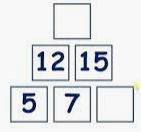
\includegraphics{Year_6_Mixed_Tests/Homework_Tasks/Addition_pyramid_1.png}
\end{center}

\\

\item \quad \( \framebox(50,15){} + 3,874 = 4,102 \) \vspace{5pt} \\

\item \quad \( 87,302 = 25,238 + \framebox(50,15){} \) \vspace{5pt} \\

\item \quad \( 2,452 + 328 = 351 + \framebox(50,15){} \) \vspace{5pt} \\

\item \quad \( \framebox(50,15){} \div 8 = 74  \) \vspace{5pt} \\

\item \quad \( \framebox(50,15){} \times 9 = 2493  \) \vspace{5pt} \\

\item \quad \( 4^{2} - 2^{3} + 3^{2}  \) = \framebox(50,15){} \vspace{5pt} \\

\item \quad Sort the given numbers into the Venn diagram below. Numbers that fit in both circles should be put at the point of intersection (the central oval). Numbers that do not belong to any circle should be put in the sample space (between the rectangle and the circles).\hspace{1cm} \( { 2, 11, 14, 5, 6, 7} \)

\begin{center}
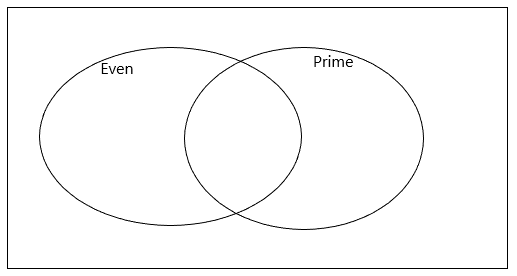
\includegraphics[width=8.5cm]{Year_6_Mixed_Tests/Homework_Tasks/Venn_Even_Prime_21_11_23_.png}
\end{center}



\end{enumerate}

\end{document}